%MATLink documentation info page
%R. Menon
\documentclass[class=minimal,border=0pt]{standalone}
\usepackage{tikz,fontspec}
\setmonofont{Menlo}
\setsansfont{OpenSans}
\setmainfont{Open Sans Condensed Bold}
\newfontfamily\oscl[LetterSpace=-2.0]{Open Sans Condensed Light}
\usetikzlibrary{mindmap, arrows, shapes, calc}
\definecolor{blue}{rgb}{0., 0.364706, 0.654902}

\begin{document}
\fontsize{13pt}{16pt}\selectfont
\tikzstyle{line}=[ultra thick, blue!70, >=stealth, rounded corners]
\tikzstyle{circ}=[circle, draw, ultra thick, lightgray!70]
\tikzstyle{rect}=[rectangle, blue!70, draw, ultra thick, rounded corners]
\tikzstyle{connect}=[circle connection bar switch color=from (lightgray!70) to (blue!70)]

\begin{tikzpicture}
	\node (mma) [circ, anchor=west] at (current page.west) {
\includegraphics[width=1.5in]{mma}};
	\node (matlink) [circ, blue!70, anchor=west, shift={(4,0)}] at (mma.east) {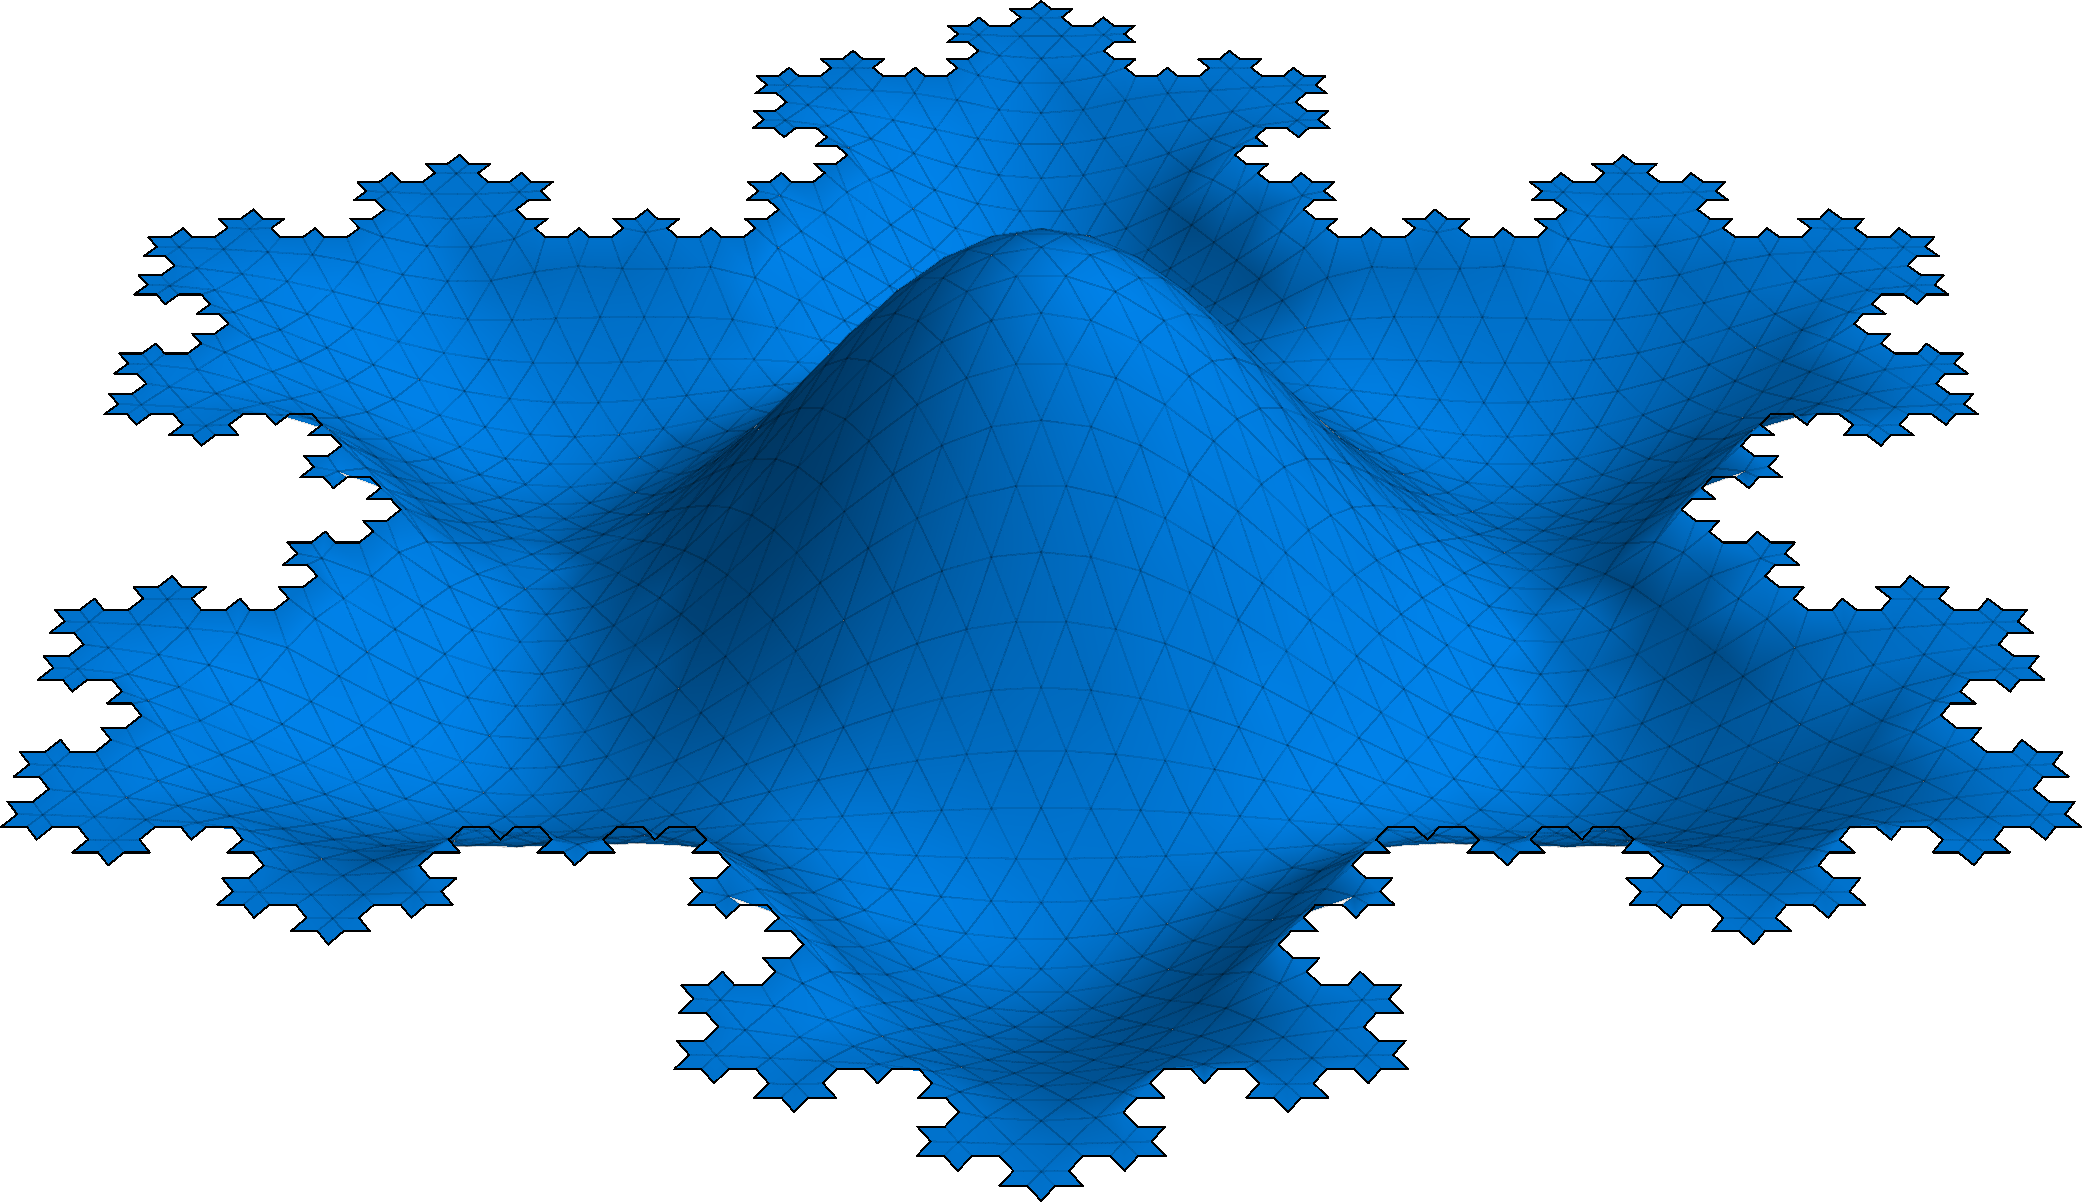
\includegraphics[width=3in]{matlink}};
	\node (matlab) [circ, anchor=west, shift={(6,0)}] at (matlink.east) {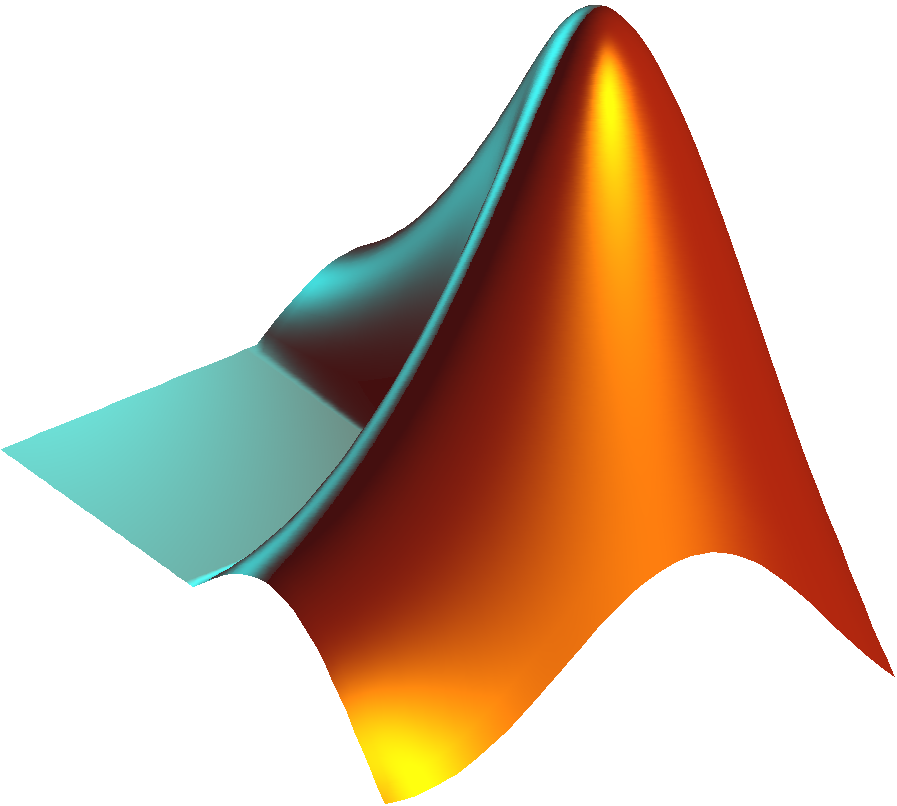
\includegraphics[width=1.5in]{matlab}};

	\node (needs) [rect, minimum width=5.5cm, anchor=center, shift={(1,6)}] at (mma.east) {
		\begin{minipage}{4.5cm}
			\begingroup
				\fontsize{18pt}{21pt}\selectfont
				{\color{blue}{Load Application}}\\[0.2in]
			\endgroup
			\color{black}
			\texttt{Needs["MATLink`"]}
		\end{minipage}
	};

	\node (funcs) [rect, minimum width=8cm, anchor=center, shift={(0,-3)}, align=center] at (matlink.south) {
		\begin{minipage}{6.9cm}
			\begingroup
				\fontsize{18pt}{21pt}\selectfont
				{\color{blue}{
				{\oscl\textbf{\emph{Mathematica}}} Interface}}\\
			\endgroup
			\color{black}
			\begin{itemize}
				\item \texttt{MEvaluate, MSet, MGet,}
				\item \texttt{MScript, MFunction, MCell}
				\item \texttt{CommandWindow, MATLABCell}
			\end{itemize}
		\end{minipage}
	};

	\node (mengine) [rect, minimum width=5.5cm, anchor=center, shift={(3.5,6)}] at (matlink.east) {
		\begin{minipage}{4.5cm}
			\begingroup
				\fontsize{18pt}{21pt}\selectfont
				{\color{blue}{MATLAB Engine}}\\
			\endgroup
			\color{black}
			\begin{itemize}
				\item \texttt{ConnectEngine}
				\item \texttt{DisconnectEngine}\\
				\item \texttt{OpenMATLAB}
				\item \texttt{CloseMATLAB}
			\end{itemize}
		\end{minipage}
	};


	\draw [<-, line] (mma.north) |- (needs.west);
	\draw [-, line] let \p1=($(needs.east)-(matlink.120)$),\n1={\y1/sin(120)} in (matlink.120)--++(120:\n1) -- (needs.east);

	\draw [<-, line] (mma.south) |- (funcs.west);
	\draw [->, line] (funcs.east) -| (matlab.south);

	\draw [->, line] (mengine.east) -| (matlab.north);
	\draw [-, line] let \p1=($(mengine.west)-(matlink.60)$),\n1={\y1/sin(60)} in (matlink.60)--++(60:\n1) -- (mengine.west);

	\draw [-, line] (matlink.south) to (funcs.north);

	\path (mma) to[connect] (matlink);
	\path (matlab) to[connect] (matlink);
\end{tikzpicture}
\end{document}
